Para verificar y probar correctamente la funcionalidad de los algoritmos ya sea de Fuerza Bruta o Programación Dinámica aparte de usar los casos aleatorios normales es importante obtener resultados con casos que posean ciertas características distintivas o limites respecto a los demás, es por ello que los 5 principales serán casos con cadenas con caracteres vacíos, cadenas con caracteres repetidos, cadenas simétricas, cadenas asimétricas y donde las matrices tienen un mismo valor para todas las operaciones. (Estos datasets pueden ser encontrados en sus respectivas carpetas dentro del repositorio o en el archivo)\\

1. Caso con cadenas vacías: \\
\begin{figure}[ht]
  \centering
  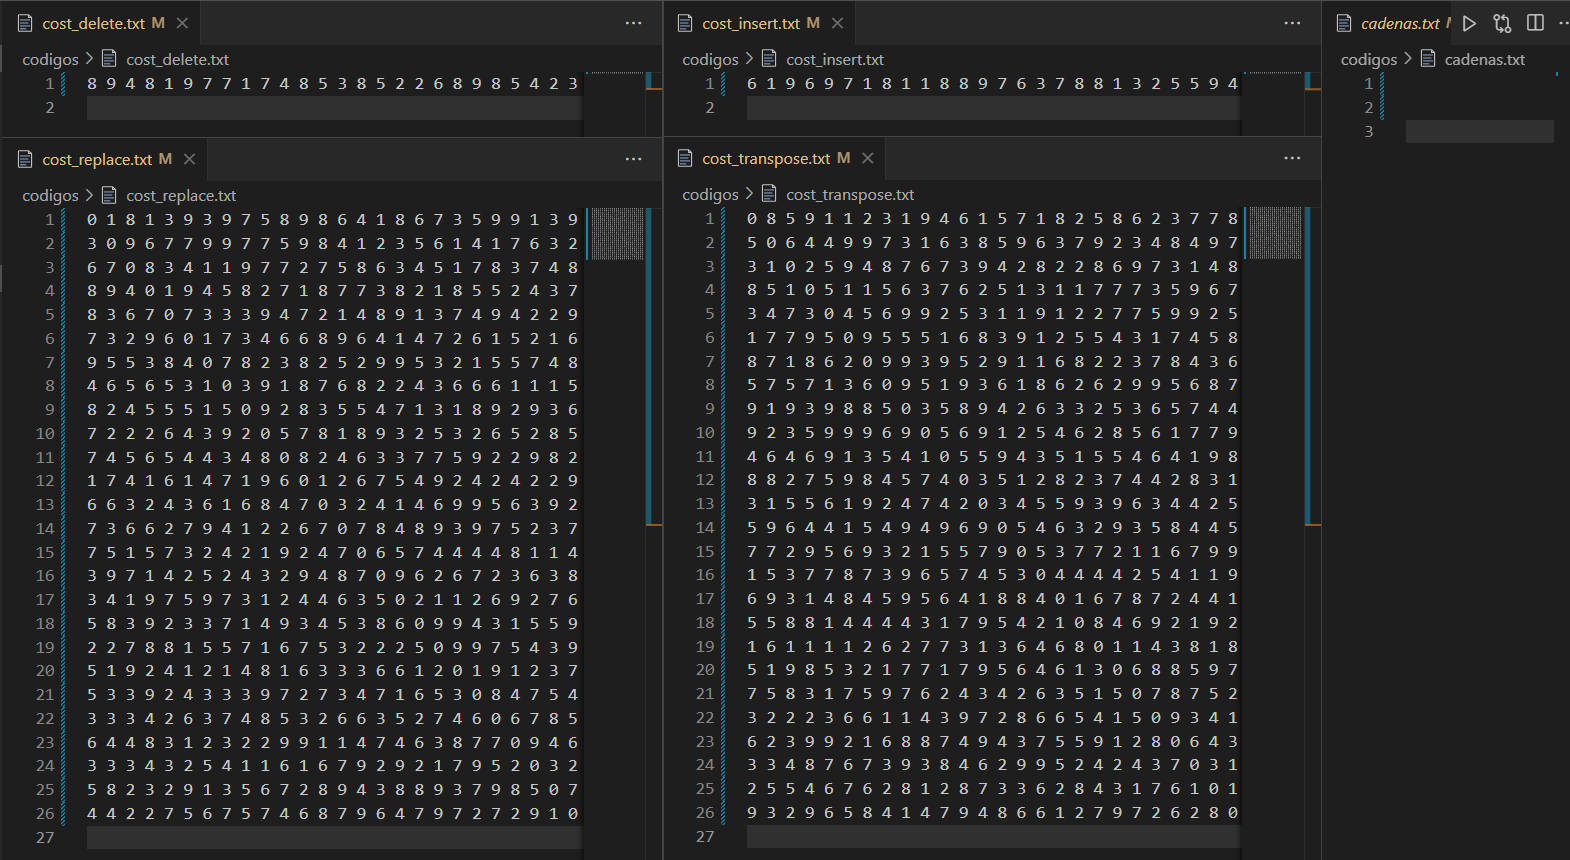
\includegraphics[width=0.8\textwidth]{./images/Casos1.png}
  \caption{Archivos con las tablas y cadenas necesarias para el caso limite 1}
  \label{fig:imagen}
\end{figure}

2. Caso con cadenas repetidas:\\
\begin{figure}[ht]
  \centering
  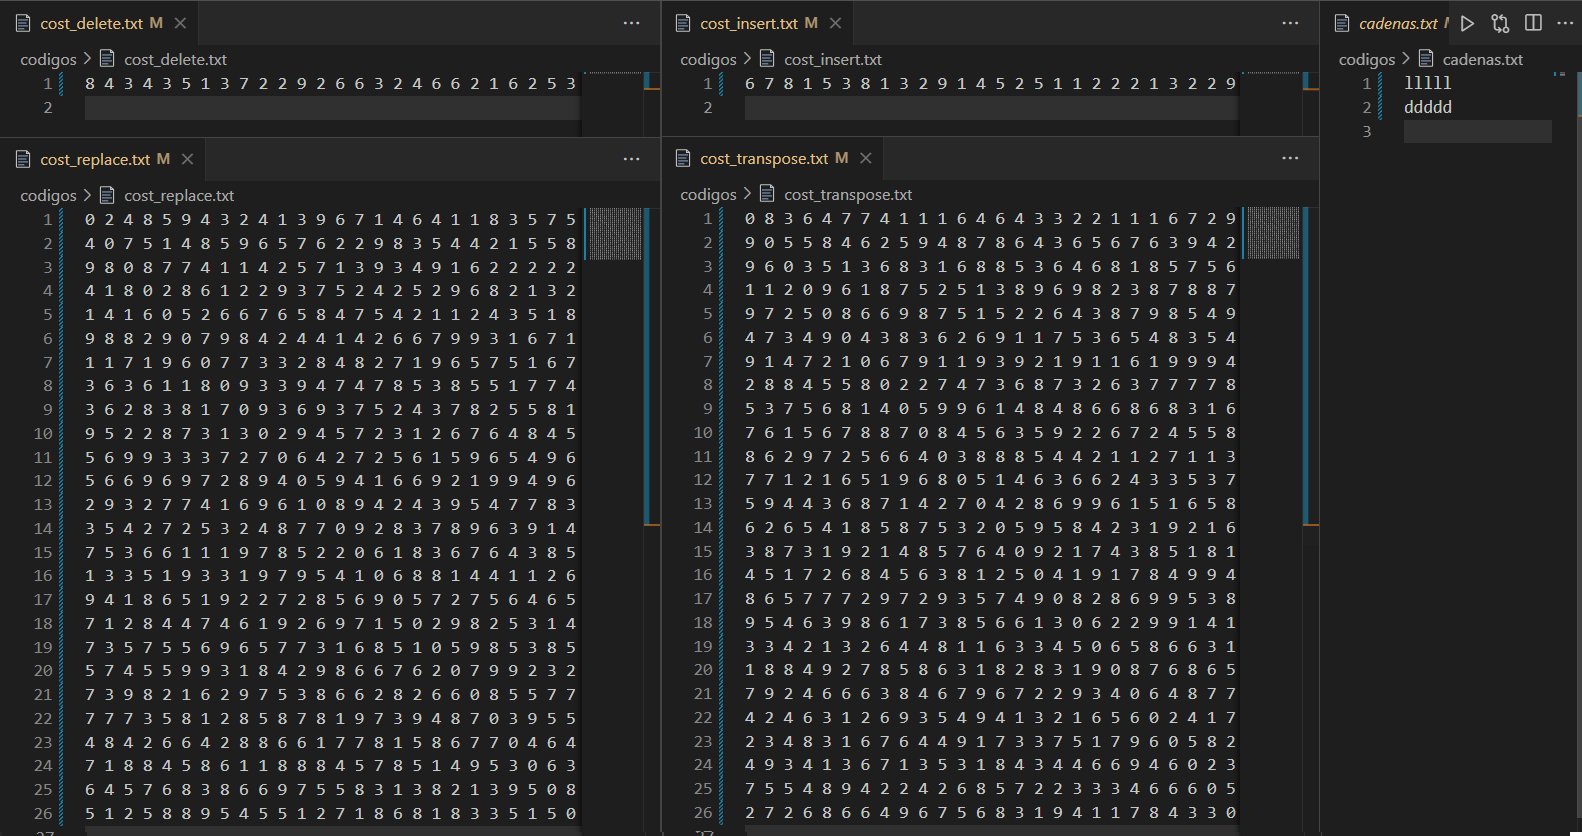
\includegraphics[width=0.8\textwidth]{./images/Casos2.png}
  \caption{Archivos con las tablas y cadenas necesarias para el caso limite 2}
  \label{fig:imagen}
\end{figure}

3. Caso con cadenas simétricas:\\
\begin{figure}[ht]
  \centering
  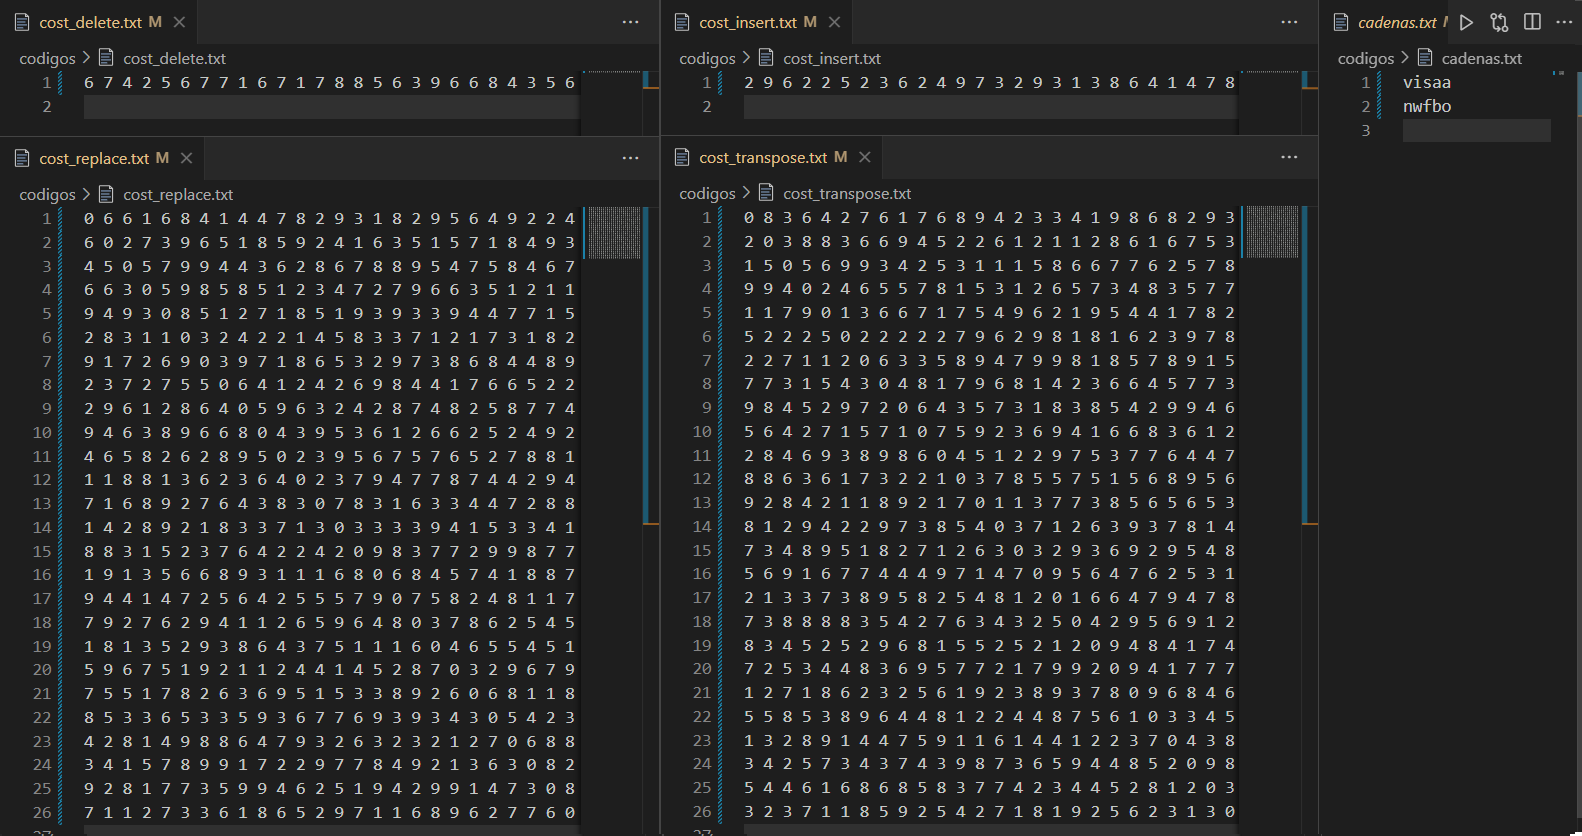
\includegraphics[width=0.8\textwidth]{./images/Casos3.png}
  \caption{Archivos con las tablas y cadenas necesarias para el caso limite 3}
  \label{fig:imagen}
\end{figure}
\newpage
4. Caso con cadenas asimétricas:\\
\begin{figure}[ht]
  \centering
  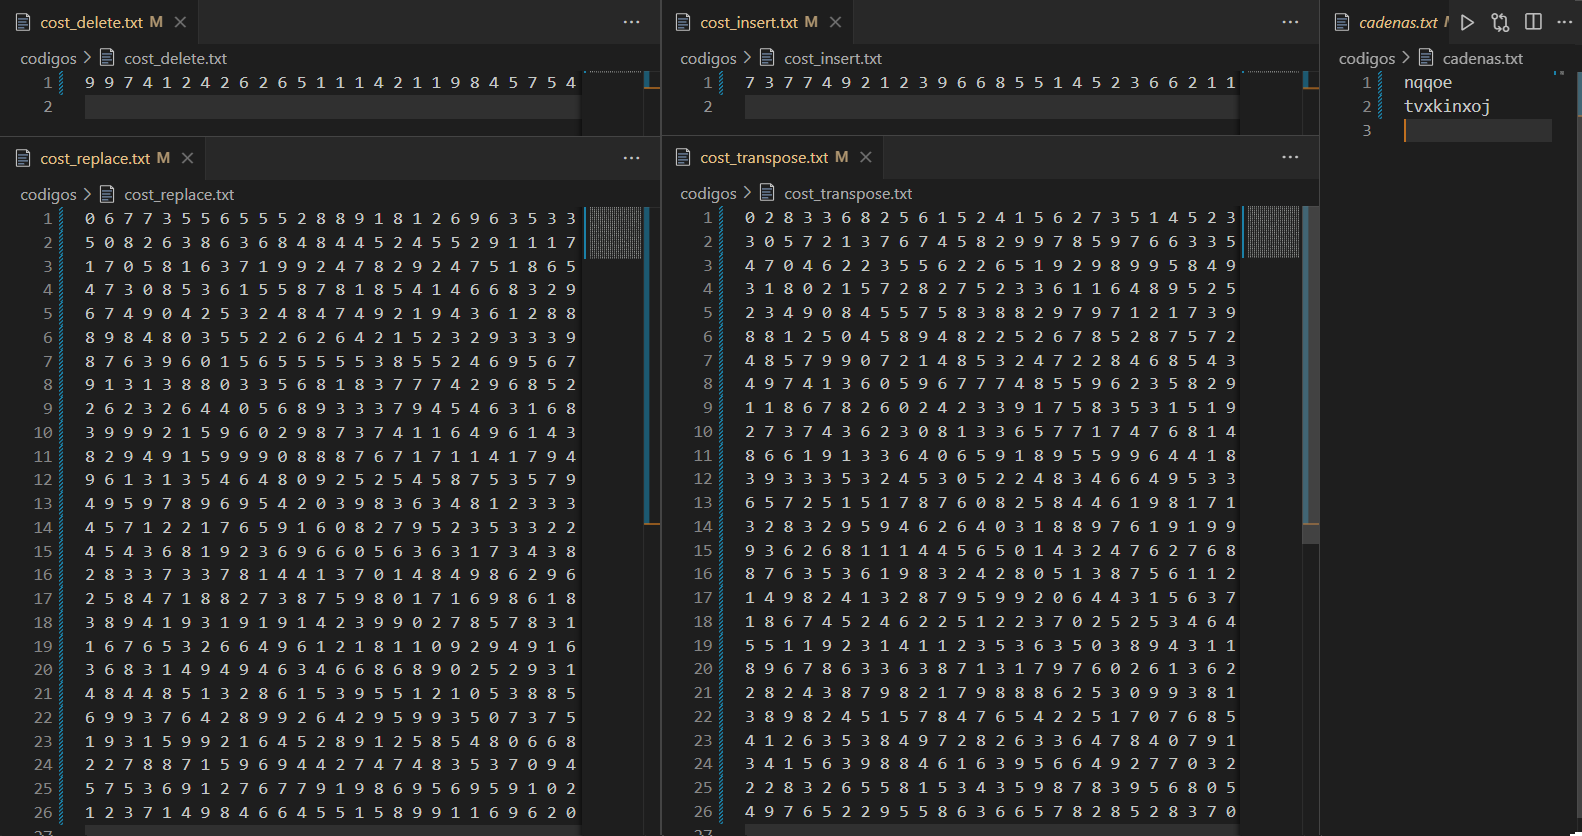
\includegraphics[width=0.8\textwidth]{./images/Casos4.png}
  \caption{Archivos con las tablas y cadenas necesarias para el caso limite 4}
  \label{fig:imagen}
\end{figure}

5. Caso con matrices con valores iguales:\\
\begin{figure}[ht]
  \centering
  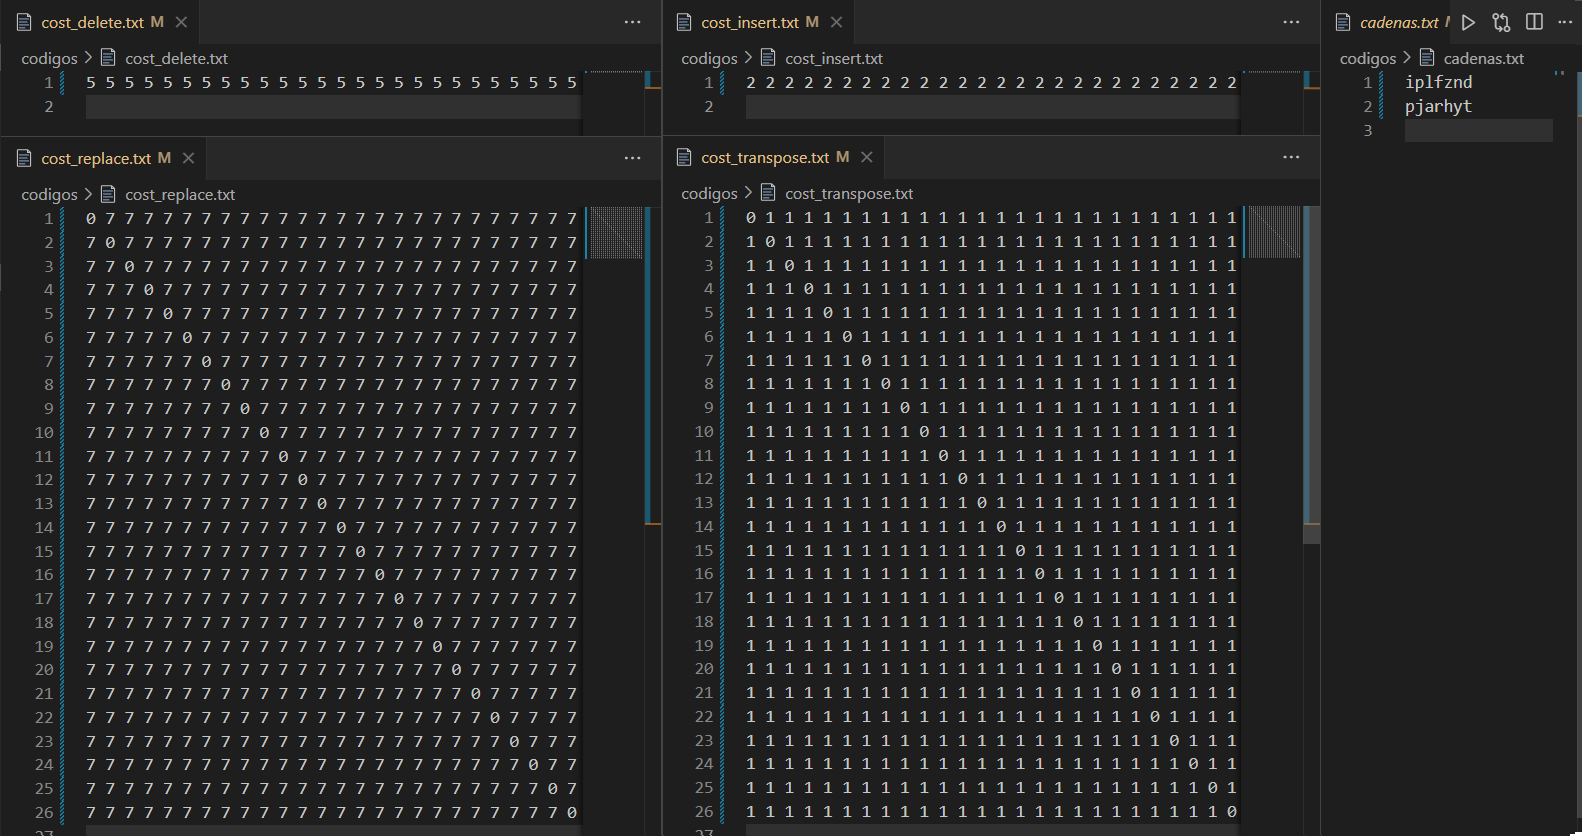
\includegraphics[width=0.8\textwidth]{./images/Casos5.png}
  \caption{Archivos con las tablas y cadenas necesarias para el caso limite 5}
  \label{fig:imagen}
\end{figure}
\newpage